\documentclass[a4paper,portrait]{scrartcl}
\author{Andreas Mai}
\title{HM I + II Zusammenfassung KIT}
\usepackage[utf8]{inputenc}
\usepackage[T1]{fontenc}
\usepackage{lmodern}
\usepackage[german]{babel}
\usepackage{graphicx}
\usepackage{amsmath}
\usepackage{amsfonts}
\usepackage{color}
\everymath{\displaystyle}
\begin{document}

\maketitle
\begin{center}
\textbf{HM Klausur am 30.08.2016} \\
\textbf{08:00 - 10:00 HM I} \\
\textbf{11:00 - 13:00 HM II} 
\end{center}

\begin{center}
\textit{Kein Anspruch auf Vollständigkeit ;)}
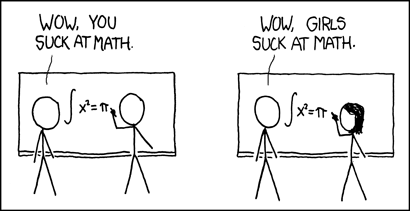
\includegraphics{how_it_works.png}

\end{center}
\clearpage
\tableofcontents
\clearpage
\setcounter{page}{1}
\section{Folgen und Reihen}
\subsection{Allgemein}
\begin{itemize}
	\item Eine Folge ist eine durchnummerierte Menge von Zahlen.  $(s_n)_{n \in \mathbb{N}}, s\in\mathbb{R}$
	\item Eine Reihe ist die Summe einer Folge.  $(s_m)_{m \in \mathbb{N}}, s\in\mathbb{R}$ \\ Eine Reihe ist auch eine Folge! $\sum_{i=1/0}^{n}(s_i),  s\in\mathbb{R}$
	\item Kleinste obere Schranke = Supremum
	\\Größte untere Schranke = Infimum
	\item Geometrische Reihe: $\sum_{i=0}^{n}q^i = \frac{q^{n+1} - 1}{q-1}, q \neq 1$
\end{itemize}
\subsection{Monotonie}
Zu faul, evtl später: https://youtu.be/Ii0b3L5UWZw

\subsection{Konvergenz}
\begin{itemize}
	\item Eine Folge (oder Reihe) ist konvergent, wenn sie gegen einen bestimmten Wert konvergiert.
	\item Sie ist bestimmt divergent, wenn sie gegen $ \pm  \infty $ läuft
	\item Sie ist unbestimmt divergent, wenn sich keine Aussage machen lässt \\ (bsp: 1 und -1 abwechseln).
	\item Formel: $\forall \varepsilon > 0: \exists n_0: \forall n \geq n_0: |s_n - g| < \varepsilon$ ($g$: Grenze)
\end{itemize}
\subsubsection*{Grenzwert bestimmen}
Grad der Funktion:
\begin{itemize}
  \item $Zählergrad < Nennergrad \Rightarrow  s_{n} \rightarrow 0$ \\
  Beispiel: $s_{n} = \frac{n}{n^2+4} \Rightarrow s_{n} \rightarrow 0$
  \item $Zählergrad = Nennergrad \Rightarrow  s_{n} \rightarrow Bruch$ \\
    Beispiel: $s_{n} = \frac{3n+4}{5n+96} \Rightarrow s_{n} \rightarrow \frac{3}{5}$
  \item $Zählergrad > Nennergrad \Rightarrow  s_{n} \rightarrow \infty \Rightarrow $ bestimmt divergent \\
    Beispiel: $s_{n} = \frac{n^6-7}{n^2+4} \Rightarrow s_{n} \rightarrow \infty$
\end{itemize}
\subsubsection*{Grenzwert beweisen}
Durch Formel.
\subsubsection*{Beispiel}
$ s_n = \frac{1}{n} $ \\
Zählergrad < Nennergrad $\Rightarrow  s_{n} \rightarrow 0$ \\
$ |s_n - g| = |\frac{1}{n} - 0| = \frac{1}{n} < \frac{1}{n_0} \leq \varepsilon$ \\
Drüber schreiben: Es sei $n_0 > \frac{1}{\varepsilon}$
\subsubsection{Nullfolgenkriterium}
\subsubsection{Mino/Majorantenkriterium}
\subsubsection{Cauchykriterium}
\subsubsection{Leibnitzkriterium}
https://youtu.be/xOhr3rFTjok
\subsubsection{Noch son kack Kriterium}
\subsection{Koshere Folgen (Cauchy-Folgen)}
Jede Konvergente Folge ist eine Cauchy Folge und ungekehrt.\\
Hier steht fast das gleiche wie unter Konvergenz\\
Sinn: Ab einem Mindestindex $n_0$ ist der Abstand zwischen 2 Folgegliedern kleiner als $\varepsilon$
\subsubsection*{Formel}
$ \forall \varepsilon > 0 \exists n_0 \forall n,m > n_0: |s_n - s_m| < \varepsilon$

\section{Differenzieren (Ableiten)}

\section{Integrieren}
\subsection{Partielle Integration}
Verwendung: Integration von Produkten (z.B. $ \int \! x \cdot e^x \, \mathrm{d}x $)
\subsubsection*{Formel}
$ \int f'(x) \cdot g(x) \mathrm{d}x = f(x) \cdot g(x) - \int f(x) \cdot g'(x) \, \mathrm{d}x$
\subsubsection*{LAPTE}
\textbf{L}ogarithmisch, \textbf{A}lgebraisch/\textbf{P}olynom, \textbf{T}rigonometrisch, \textbf{E}xponential \\
Linke Funktion ableiten $g \rightarrow g'$ und rechte integrieren $f'\rightarrow f$ (links $g$, rechts $f'$)
\subsubsection*{Beispiel}
$ \int \! x \cdot e^{2x} \, \mathrm{d}x$ \\
$\Rightarrow$ durch LAPTE: $f'(x) = e^{2x}, g(x) = x$ \\
$\Rightarrow f(x) = \frac{1}{2} e^{2x}, g'(x) = 1 $  \\
Aus der Formel folgt: 
$ \int \! x \cdot e^{2x} \, \mathrm{d}x = \frac{1}{2} e^{2x} \cdot x - \int \! \frac{1}{2} e^{2x} \, \mathrm{d}x = \frac{1}{2} e^{2x} \cdot x - \frac{1}{4} e^{2x} = \frac{1}{4} e^{2x} \cdot (2x-1)$
\subsection{Substitution}
Verwendung: Keine ahnung, dann wenn mans braucht. denk und rechne!
\subsubsection*{Formel}
$ \int_{\varphi(a)}^{\varphi(b)} \! f(x) \,\mathrm{d}x = \int_{a}^{b} \! f(\varphi(t)) \cdot \varphi'(t) \,\mathrm{d}t$
\subsubsection*{Beispiel}
$ \int_{1}^{2} \!(x^2+2)^3 \cdot 2x \,\mathrm{d}x $ \\
Setze $ u = x^2 + 2 \Rightarrow \mathrm{d}u = 2x \,\mathrm{d}x \Rightarrow \mathrm{d}x = \frac{\mathrm{d}u}{2x}$ \\
$ \int \!(x^2+2)^3 \cdot 2x \,\mathrm{d}x = \int \! u^3 \,\mathrm{d}u = \frac{1}{4}u^4 = \frac{1}{4}(x^2+2)^4$ \\
Grenzen einfügen: $ \int_{1}^{2} \!(x^2+2)^3 \cdot 2x \,\mathrm{d}x = \left[ \frac{1}{4}(x^2+2)^4 \right]_1^2 = \frac{1}{4}(2^2+2)^4 - \frac{1}{4}(1^2+2)^4 = \frac{1}{4}6^4 - \frac{1}{4}3^4$
\subsubsection*{Weiteres Beispiel}
$ \int \!cos(x^3) \cdot 6x^2 \,\mathrm{d}x $ \\
Setze $ u = x^3 \Rightarrow \mathrm{d}u = 3x^2 \,\mathrm{d}x \Rightarrow \mathrm{d}x = \frac{\mathrm{d}u}{3x^2}$ \\
$ \int \!cos(u) \cdot 6x^2 \cdot \frac{\mathrm{d}u}{3x^2} = \int \!cos(u) \cdot 2 \,\mathrm{d}u = 2 \int \!cos(u) \,\mathrm{d}u = 2 sin(u) = 2 sin(x^3)$
\end{document}
